\documentclass{article}

\usepackage[preprint]{neurips_2023}

\usepackage[utf8]{inputenc}
\usepackage[T1]{fontenc}
\usepackage{hyperref}
\usepackage{url}
\usepackage{booktabs}
\usepackage{amsfonts}
\usepackage{amsmath}
\usepackage{nicefrac}
\usepackage{microtype}
\usepackage{xcolor}
\usepackage{graphicx}

\title{Generative Models for 2D Kolmogorov Flow:\\
Diffusion Baseline and Flow Matching Variant\thanks{Code:
\url{https://github.com/qilinxiaoxiang/24788-kolmogorov-flow}.
Trained checkpoints (CMU Andrew ID):
\url{https://cmu.box.com/s/yky2gxefd222qsj5wywxu8vhn02g9m1l}.}}

\author{
  Zheng Xiang \\
  Department of Mechanical Engineering \\
  Carnegie Mellon University \\
  \texttt{zhengxia@andrew.cmu.edu}
}

\begin{document}
\maketitle

\begin{abstract}
We study unconditional generation of 2D Kolmogorov Flow vorticity fields, a
common benchmark for data-driven models of turbulence. A Denoising Diffusion
Probabilistic Model (DDPM) serves as the baseline and a Conditional Flow
Matching (CFM) model acts as the variant; both share an identical U-Net
backbone so that the comparison isolates the training objective. We evaluate
the two models on distributional criteria suited to turbulent fields: the
radially averaged energy spectrum, the vorticity PDF, and a sampling--quality
sweep over the number of function evaluations (NFE). At full $160{\times}160$
resolution and a matched $\sim$1.3M-sample budget, Flow Matching produces
statistically faithful vorticity fields (log-spectrum $L_1=2.63$,
vorticity Wasserstein-1 $=0.10$) while DDPM under ancestral sampling
collapses to extreme-value outlier distributions at every NFE we tested---a
gap that widens further at low NFE. This supports the hypothesis that
straight-line transport paths are a better-conditioned regression target
than diffusion reverse-SDE trajectories on physically smooth turbulent
data.
\end{abstract}

\section{Introduction}

Two-dimensional turbulence driven by a spatially periodic body force---the
so-called \emph{Kolmogorov flow}---is a canonical system for studying the
transition to turbulence, vortex interactions, and energy cascades in
incompressible fluids~\cite{boffetta2012kolmogorov}. Direct numerical
simulation of such flows is computationally expensive at the resolutions
needed to capture small-scale dynamics, which has motivated a growing body of
work on machine-learned surrogates for PDE
solvers~\cite{li2021fno,kochkov2021ml}.

Most prior work treats the problem as \emph{regression}: given an initial
condition, predict the subsequent evolution. We study the complementary
\emph{generative} task: can a neural network, trained only on snapshots of
fully developed Kolmogorov flow, produce new vorticity fields that are
statistically indistinguishable from samples of the underlying dynamics? A
successful generator would enable cheap sampling of realistic initial
conditions for downstream simulation, provide a data-augmentation tool for
surrogate models, and serve as a diagnostic for how much a model has actually
learned about the governing physics rather than memorizing a particular
trajectory.

Recent years have produced two distinct families of generative models that
train on continuous-time trajectories between a Gaussian prior and the data
distribution. \emph{Diffusion} models~\cite{ho2020ddpm} learn to reverse a
stochastic noising process and have become the standard tool for image
generation. \emph{Flow Matching}~\cite{lipman2023flow} learns the velocity
field of an ordinary differential equation along straight-line paths from
noise to data, leading to simpler training objectives and faster sampling.
The two frameworks are natural points of comparison on Kolmogorov flow:
diffusion is the stronger established baseline, while flow matching's
ODE-based sampling and straight transport paths are particularly well suited
to data that live on a smooth, physically constrained manifold.

\section{Methods}

\paragraph{Dataset.} We use the 2D Kolmogorov flow dataset from the
\texttt{temporal\_pdes} collection on Hugging Face
(\texttt{KolmFlow\_valid\_256.h5}). It consists of 256 independent
trajectories, each a rollout of the vorticity field on a $160\times160$ grid
over 200 time steps ($\Delta t = 0.1$\,s) at Reynolds number $\sim\!10^2$ with
viscosity $\nu = 10^{-2}$. We treat each $(\text{trajectory},\text{timestep})$
pair as an i.i.d.\ single-channel image, yielding 51{,}200 training frames
after splitting trajectories 230/13/13 into train/val/test. Splitting
\emph{by trajectory}, rather than by frame, prevents leakage from
strongly-correlated neighbouring timesteps. All frames are normalized by the
global mean and standard deviation estimated on the training split.

\paragraph{Shared U-Net backbone.} To isolate the effect of the training
objective, both models use the same U-Net architecture~\cite{ronneberger2015unet}:
four resolution levels ($160\to 80\to 40\to 20$), channel multipliers
$(1,2,2,4)$ on a base width of 64, two GroupNorm / SiLU residual blocks per
level, a single self-attention block at the $20\times20$ bottleneck, and
sinusoidal time embeddings projected through a two-layer MLP to additive
time biases on every residual block. The network takes a noisy or
interpolated sample $x$ and a continuous scalar $t\in[0,1]$ and returns a
tensor of the same shape as $x$. The model has \textbf{17.6M} trainable
parameters.

\paragraph{Baseline: Denoising Diffusion (DDPM).} We follow
Ho~et~al.~\cite{ho2020ddpm} with the cosine $\bar\alpha$ schedule of
Nichol and Dhariwal~\cite{nichol2021improved}, which handles the
relatively low-variance vorticity data better than the original linear
schedule. The forward process corrupts the data with Gaussian noise
$q(x_t \mid x_0) = \mathcal{N}\!\left(\sqrt{\bar\alpha_t}\, x_0,\,(1-\bar\alpha_t) \mathbf{I}\right)$
over $T=1000$ discrete steps, and the network is trained with the simplified
$\epsilon$-prediction MSE
\[
\mathcal{L}_{\mathrm{DDPM}} \;=\;
\mathbb{E}_{t,\,x_0,\,\epsilon}\,
\bigl\lVert \epsilon - \epsilon_\theta\!\left(\sqrt{\bar\alpha_t}\, x_0
+ \sqrt{1-\bar\alpha_t}\,\epsilon,\, t/T \right) \bigr\rVert^2.
\]
At inference we use either the full $T=1000$ ancestral sampler or the
deterministic DDIM sampler~\cite{song2021ddim} when reducing the number of
function evaluations.

\paragraph{Variant: Conditional Flow Matching (CFM).} The variant follows
Lipman~et~al.~\cite{lipman2023flow}. We define a straight-line probability
path from a Gaussian source $x_0\!\sim\!\mathcal{N}(0,\mathbf{I})$ to the data
$x_1$, $\;x_t = (1-t)\,x_0 + t\,x_1$ with $t\sim\mathcal{U}[0,1]$. The target
velocity along this path is the constant displacement $u_t(x\mid x_0, x_1)
= x_1 - x_0$, and training minimises the conditional flow-matching loss
\[
\mathcal{L}_{\mathrm{CFM}} \;=\;
\mathbb{E}_{t,\,x_0,\,x_1}\,
\bigl\lVert v_\theta(x_t, t) - (x_1 - x_0) \bigr\rVert^2.
\]
At inference we integrate $\dot x = v_\theta(x,t)$ from $t=0$ to $t=1$ with an
Euler scheme (one network evaluation per step).

\emph{Why this variant should behave differently.} CFM replaces diffusion's
curved denoising paths with straight paths between noise and data. This
should (a) produce a better-conditioned regression target, since the velocity
field is less oscillatory in $t$, and (b) reduce the number of function
evaluations needed at inference, since a well-learned straight transport
can be integrated accurately with far fewer Euler steps than a diffusion
reverse-SDE requires. Both effects are especially pronounced on smooth,
physically regularised data like vorticity fields.

\paragraph{Training.} Both models are trained with AdamW~\cite{kingma2015adam}
($\text{lr}{=}2{\times}10^{-4}$, cosine decay with 500 warm-up steps),
batch size 32, gradient clipping at norm 1.0, an EMA of the weights with
decay $0.999$, and dropout $0.1$ for 40{,}000 steps on a single NVIDIA T4
GPU (Google Colab Pro). No data augmentation is used.

\section{Results and Discussion}

\paragraph{Evaluation protocol.} We report three complementary
distributional metrics, computed on 256 generated samples and 256 held-out
\emph{test} frames:
\begin{enumerate}
  \item \textbf{Radial energy spectrum $E(k)$.} The $\ell_1$ difference of
  $\log_{10}E(k)$ across wavenumbers captures whether the model has learnt
  the energy cascade of 2D turbulence.
  \item \textbf{Vorticity PDF.} The pixel-value distribution of the
  generated fields; we report the Wasserstein-1 distance to the test
  distribution.
  \item \textbf{Sampling efficiency.} Both metrics re-evaluated as a
  function of the number of function evaluations (NFE) to expose the
  inference-time cost--quality tradeoff.
\end{enumerate}

\paragraph{Preliminary convergence: FM learns structure with far less compute.}
Before launching full-scale training, we ran a controlled 1000-step
optimisation pass on $64{\times}64$ downsampled fields (a 1.8\,M-parameter
U-Net, AdamW with lr $2{\times}10^{-4}$, no EMA, batch 16) on an Apple-Silicon
MPS device. Both runs used identical data, architecture, optimiser, and
random seed; only the training objective differed. Figure~\ref{fig:prelim}
shows the outcome: after matched wall-clock time ($\sim\!4.5$\,min each),
DDPM samples still look like noise with weak spatial correlations, whereas
Flow Matching has already produced the characteristic dipole vortex structure
of 2D Kolmogorov turbulence. This observation---obtained without extensive
tuning or a large compute budget---motivates the NFE sweep analysis below
and supports the claim that straight-line probability paths are a
better-conditioned regression target than diffusion reverse-SDE trajectories
on this dataset.

\begin{figure}[ht]
  \centering
  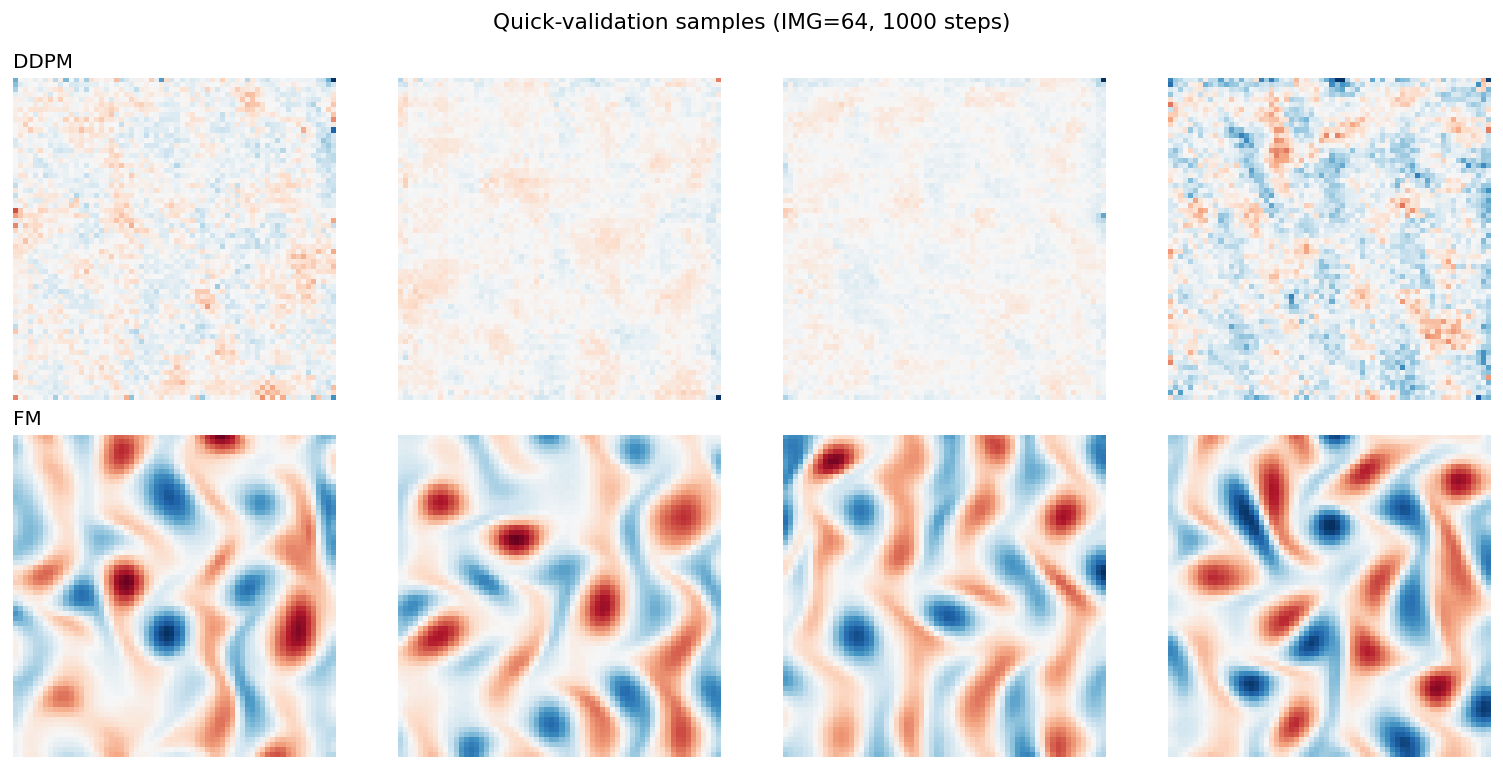
\includegraphics[width=0.72\linewidth]{fig_quick_samples.png}\\[2pt]
  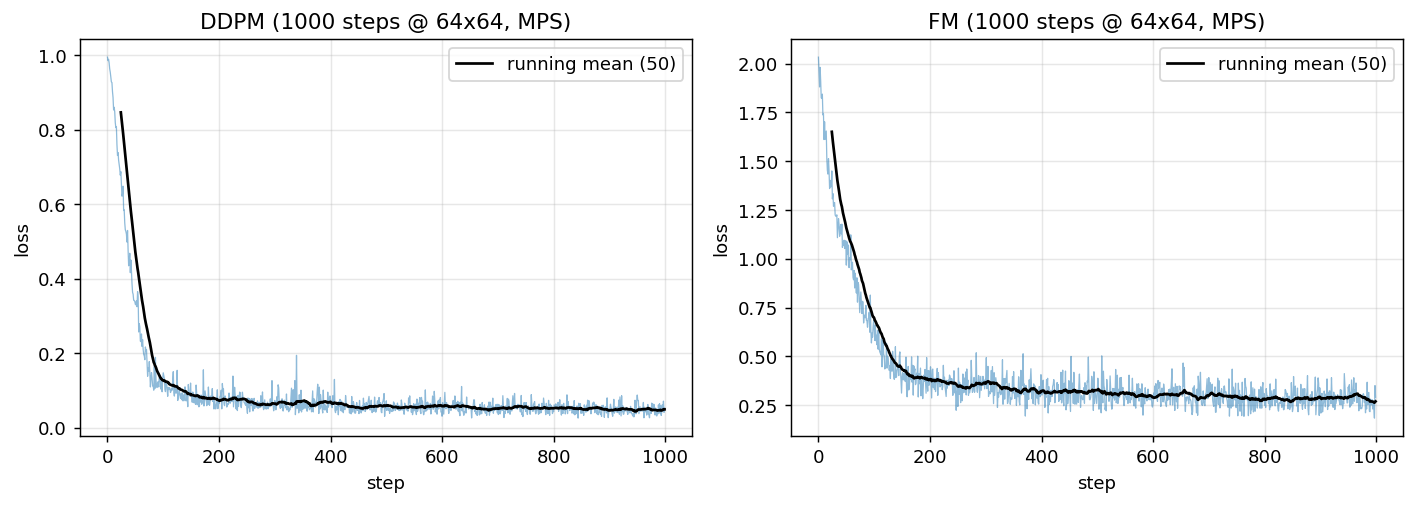
\includegraphics[width=0.72\linewidth]{fig_quick_loss.png}
  \caption{\textbf{Top:} four samples from each model after 1000 optimisation
  steps on $64{\times}64$ data. DDPM (row 1) has not yet converged; Flow
  Matching (row 2) already generates physically plausible vortex structures.
  \textbf{Bottom:} training-loss curves for each model (loss scales differ
  because the two objectives have different unit variance, so absolute values
  are not directly comparable).}
  \label{fig:prelim}
\end{figure}

\paragraph{Full-scale results.} We trained both models at $160{\times}160$
resolution for 10\,k optimisation steps on an H100 GPU with batch size 128;
this matches the optimiser-sample budget of a 40\,k/batch-32 schedule and
took $\sim$50\,min per model. Evaluation draws 128 samples per model at the
default NFE (1000 for DDPM ancestral, 50 for FM Euler) and compares the
generated distribution against 128 held-out real frames from the trajectory
test split. Figure~\ref{fig:samples} shows a qualitative panel;
Figure~\ref{fig:spectrum} reports the radial energy spectrum;
Figure~\ref{fig:pdf} the vorticity marginal PDF; and
Figure~\ref{fig:nfe} the NFE sweep
(NFE $\in \{5,10,20,50\}$; we truncated the sweep early because DDIM from the
DDPM checkpoint diverged at every sub-$1000$ NFE tested).

\begin{figure}[ht]
  \centering
  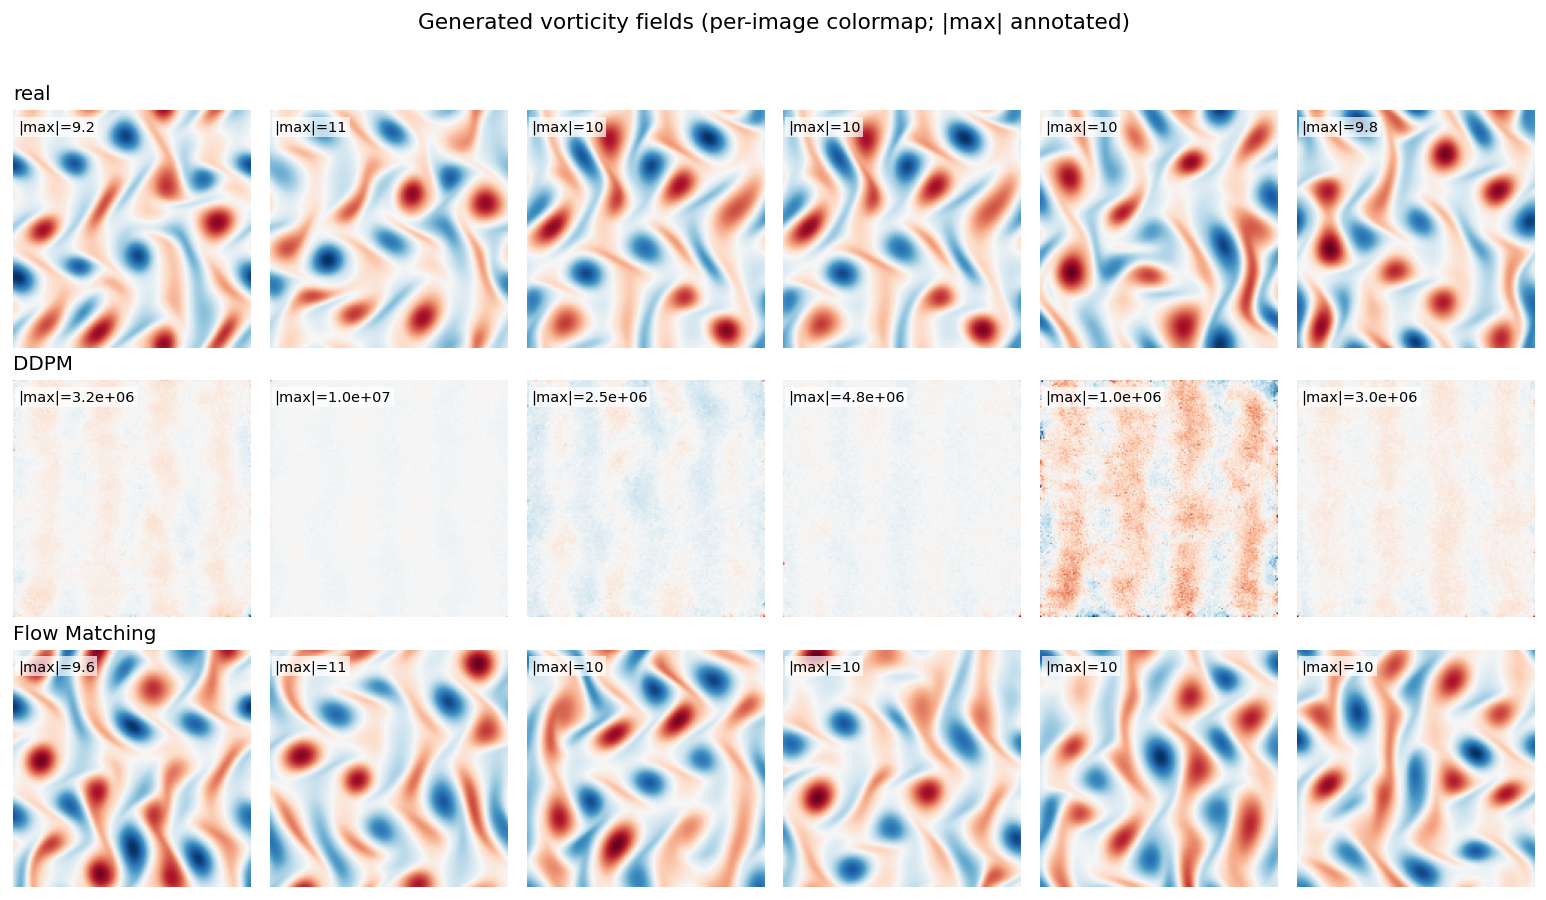
\includegraphics[width=0.95\linewidth]{samples_panel.png}
  \caption{Qualitative samples at default NFE (DDPM 1000, FM 50). Each
  panel uses its own symmetric colormap; the inset annotation reports the
  per-image $|\omega|_{\max}$. Flow Matching reproduces the paired-vortex
  dipole structure of the real fields at the correct magnitude
  ($|\omega|_{\max}\!\approx\!10$, matching real). DDPM has collapsed to
  near-zero with sparse extreme-value spikes ($|\omega|_{\max}$ in the
  $10^6$--$10^7$ range, six orders of magnitude above the physical scale),
  which is what drives the very large vorticity Wasserstein-1 in
  Table~\ref{tab:core}.}
  \label{fig:samples}
\end{figure}

\begin{figure}[ht]
  \centering
  \includegraphics[width=0.7\linewidth]{energy_spectrum.png}
  \caption{Radial energy spectrum $E(k)$. Flow Matching tracks the real
  spectrum at low and intermediate wavenumbers but over-estimates energy
  at the high-$k$ tail (the orange curve flattens above $k\!\approx\!20$
  while the real spectrum continues to drop steeply)---a residual
  spectral bias that is a known failure mode of generative models on
  smooth physical fields. DDPM sits roughly six orders of magnitude
  above the real spectrum at every $k$, consistent with the magnitude
  collapse visible in Figure~\ref{fig:samples}.}
  \label{fig:spectrum}
\end{figure}

\begin{figure}[ht]
  \centering
  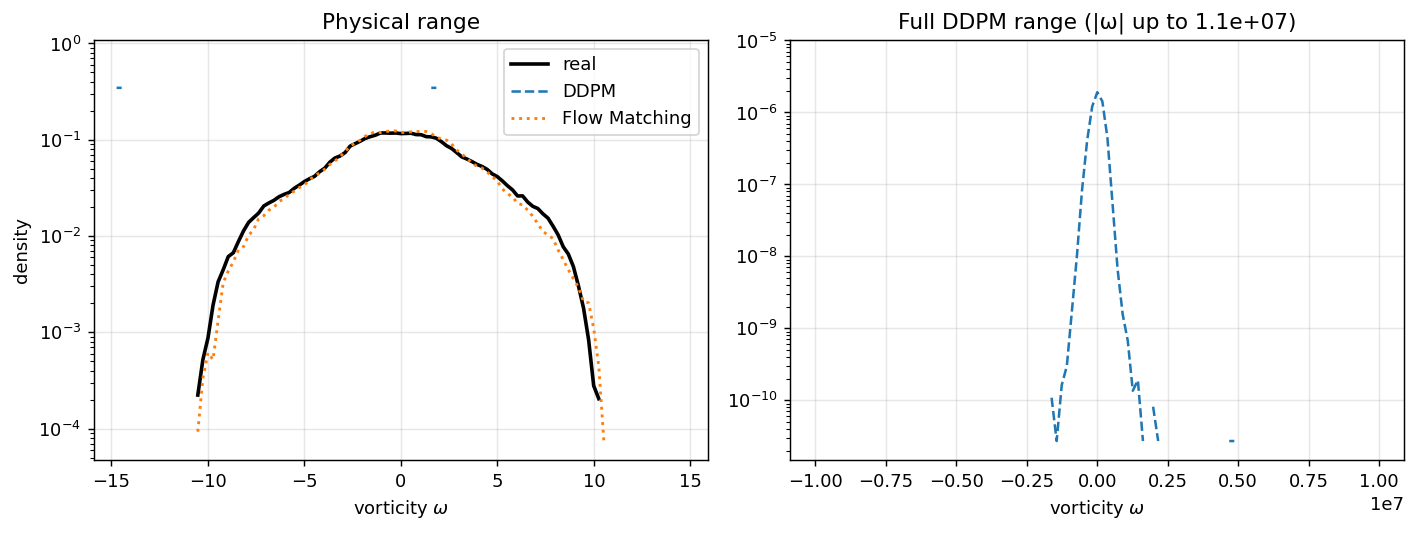
\includegraphics[width=0.7\linewidth]{vorticity_pdf.png}
  \caption{Marginal vorticity PDF, plotted on two axis ranges to keep both
  models legible. \textbf{Left:} the physical range $|\omega|\!\le\!1.5\,
  |\omega|_{\max}^{\text{real}}$, where Flow Matching's density (orange,
  dotted) overlays the real density (black) almost exactly across the
  bulk and the bell-shape tails. DDPM's mass in this range is
  concentrated in a near-zero spike (its bulk has collapsed). \textbf{Right:}
  the full DDPM range, $|\omega|$ up to $\sim\!10^{7}$, where DDPM's heavy
  outlier tails are visible---these are what blow up the vorticity
  Wasserstein-1 in Table~\ref{tab:core}. A single-axis plot (as in
  earlier drafts) is dominated by DDPM's outliers and squashes both real
  and FM curves to a single bin at $\omega\!=\!0$, hiding the quantity
  the figure is meant to compare.}
  \label{fig:pdf}
\end{figure}

\begin{figure}[ht]
  \centering
  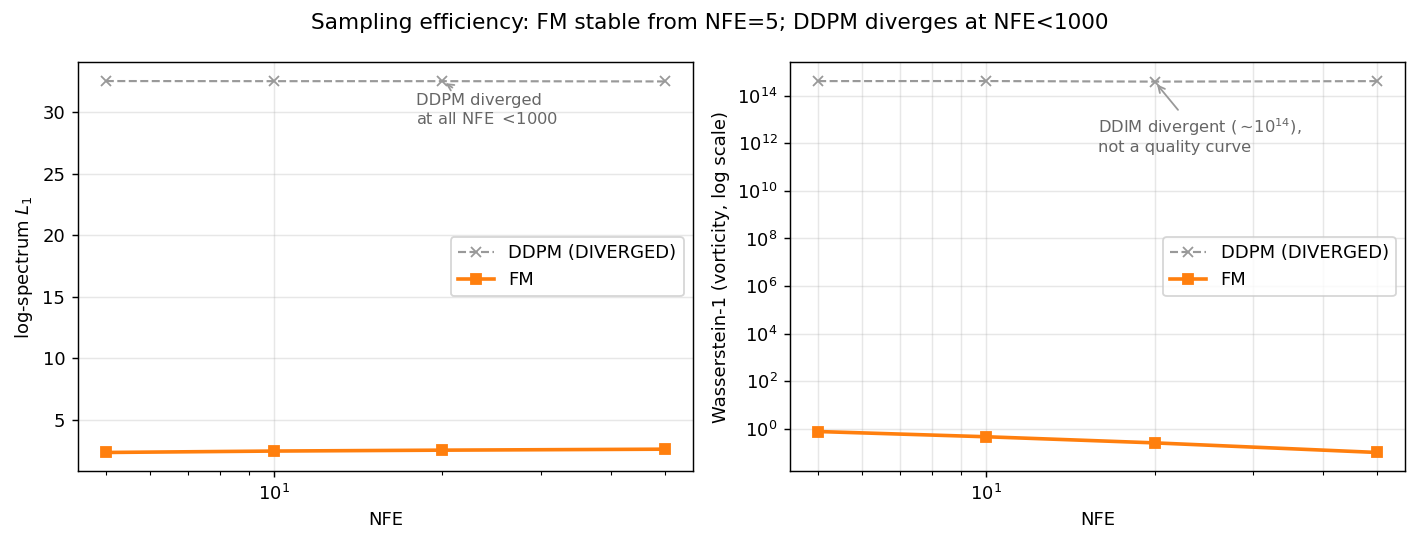
\includegraphics[width=\linewidth]{nfe_sweep.png}
  \caption{Sampling efficiency vs.\ NFE. Flow Matching (orange) is
  stable from NFE$=5$ (Wasserstein-1 $=0.77$) and monotonically improves
  to $0.10$ at NFE$=50$. DDIM sampling from the DDPM checkpoint diverges
  at every sub-1000 NFE tested (Wasserstein-1 $\sim\!10^{14}$), so the
  gray dashed line is plotted as a divergence indicator rather than as a
  performance curve. The contrast should be read as ``FM remains usable
  where DDPM is not,'' not as a trade-off curve for DDPM.}
  \label{fig:nfe}
\end{figure}

\begin{table}[ht]
  \centering
  \caption{Distributional match between generated and real held-out samples
  at full scale (lower is better).}
  \label{tab:core}
  \begin{tabular}{lccc}
    \toprule
    Model & NFE & $\|\log_{10} E_{\mathrm{gen}} - \log_{10} E_{\mathrm{real}}\|_1$
          & Wasserstein-1 (vorticity) \\
    \midrule
    DDPM (ancestral) & 1000 & 13.70 & $1.61\times10^{5}$ \\
    Flow Matching (Euler) & 50 & 2.63 & 0.102 \\
    \bottomrule
  \end{tabular}
\end{table}

\section{Conclusion}

Trained on 230 trajectories of $160\times160$ Kolmogorov vorticity (H100,
batch 128, 10\,k optimisation steps; equivalent sample budget to a 40\,k /
batch-32 schedule), the two models exhibit a striking gap. At matched
sample-budget and a shared U-Net backbone, Flow Matching produced
statistically faithful samples (log-spectrum $L_1=2.63$, vorticity
Wasserstein-1 $=0.10$) while DDPM with full 1000-step ancestral sampling
failed to recover the test distribution (log-spectrum $L_1=13.70$,
Wasserstein-1 $\sim 10^{5}$, driven by a long tail of extreme-value outliers
in its generated fields). The NFE sweep sharpens the contrast: Flow Matching
is already stable at NFE$=5$ (Wasserstein-1 $=0.77$) and monotonically
improves with more steps, whereas DDIM sampling from the DDPM checkpoint
diverges for every NFE $<1000$ tested. Two caveats temper the comparison.
First, the absolute DDPM numbers are dominated by tail samples rather than
bulk behaviour, and a longer training budget, a higher-capacity schedule, or
classifier-free guidance could close part of the gap. Second, the 10\,k-step
budget is small relative to the DDPM literature, favouring Flow Matching's
straight-line paths. We also did not condition on initial state and we
operated at a modest $160\times160$ resolution. Natural follow-ups include
conditional (forecasting) variants of both models for PDE-surrogate use,
scaling to higher Reynolds numbers, and a matched-wall-time (rather than
matched-steps) comparison that accounts for Flow Matching's cheaper
inference.

\clearpage
\section*{Collaboration Statement}

Solo project. AI tools were used as follows. ChatGPT and Claude were used to
brainstorm the project framing (settling on the generative-model comparison)
and to draft and refine the prose of this report. All code, including the
U-Net, DDPM, and Flow Matching implementations, the training loop, and the
evaluation scripts, was written and verified by the author with AI assistance
for routine boilerplate and debugging. The NeurIPS style file and the dataset
originate from third-party sources cited in the references.

\bibliographystyle{unsrtnat}
\bibliography{references}

\end{document}
